
\section{Implementation}

\subsection{Tools and versions}

The following tools and package versions was used in the implementation:

\begin{itemize}
\item GHC version 7.0.3
\item extcore version 1.0.1
\item PyPy current head branch (Last tested 09/11/2011)
\item Haskell-Python interpreter: Interpreter of Core' written in RPython
\item CPython 2.7: Used to test the Core' interpreter without it having to be correct RPython.
(pypy-python could also have been used)
\item Git was used as the projects version control system.
\end{itemize}

%\paragraph{GHC} version 7.0.3. Binary version. % Source needed for creating extcore with correct grammar file.

%\paragraph{genprimopcode} --make-ext-core-source < \{path/to/primops.txt\} > \{path/to/PrimEnv.hs\}

%\paragraph{extcore} version 1.0.1, %Source version, updated with grammar of External-core for GHC version 7.0.3 (See extcore 1.0.1 README file for details)

%\paragraph{PYPY} current head brach.

%\paragraph{Haskell-Python} interpreter of core written in RPython.


\subsection{Pipeline}

The project implements the following pipeline (see figure \ref{core2js}):
\begin{enumerate}
\item Serialize Haskell program: 
  \begin{enumerate}
  \item Create External-core file from Haskell program using GHC.
  \item Create JSCore from External-core using the extcore and JSON packages.
  \end{enumerate}
\item Deserialize JSCore:
  \begin{enumerate}
  \item Parse JSCore using the parsing tools available for PyPy
  \item Build Core AST from resulting JSON datatype
  \end{enumerate}
\item Evaluate program:
  \begin{enumerate}
  \item Evaluation is done by the already implemented PyPy Core' interpreter,
  Haskell-Python. Additional functionality had to be built on top of this, mostly 
  Haskell library functions.
  \end {enumerate}
\end{enumerate}

\subsection{Organization}

The implementation is organized as represented by figure \ref{organization}. The
main folder (interpreter) contains the main program, and a program for generating
dot\footnote{ A dot file is a file written in dot-language, used by the \emph{dot} 
command line tool from the graphviz software package}
files, "makegraph.py" (used to create graphs of parsed JSCore files using 
graphviz\footnote{ Graphviz is an open source software package for graph 
visualization}). The "haskell" folder contains the Haskell-Python Core' 
interpreter code, used by the main program for evaluation, 
and by the parser to generate the abstract-syntax-tree (AST). In addition to this,
the subfolder "ghc" implements some simple functionality to be used by the test-programs.
Among others, a very simple IO function for printing text to the terminal (putStrLn).
These are categorised into packages corresponding to GHC packages, and libraries, 
corresponding to the libraries in the GHC packages.
The RPython modules in these "packages" are loaded, and references to the attributes
they contain are used during
the creation of the AST. See figure \ref{core2js} for a simple description of the pipeline.

The "core" folder contains a Haskell program for generating JSCore files from External-core files
(core2js.hs), the JSCore parser (parser.py), and a simple datastructure representing Core modules
(module.py).

The "tests" folder naturally contains tests, each test is in its own subfolders.

\begin{figure}[H]
\centering
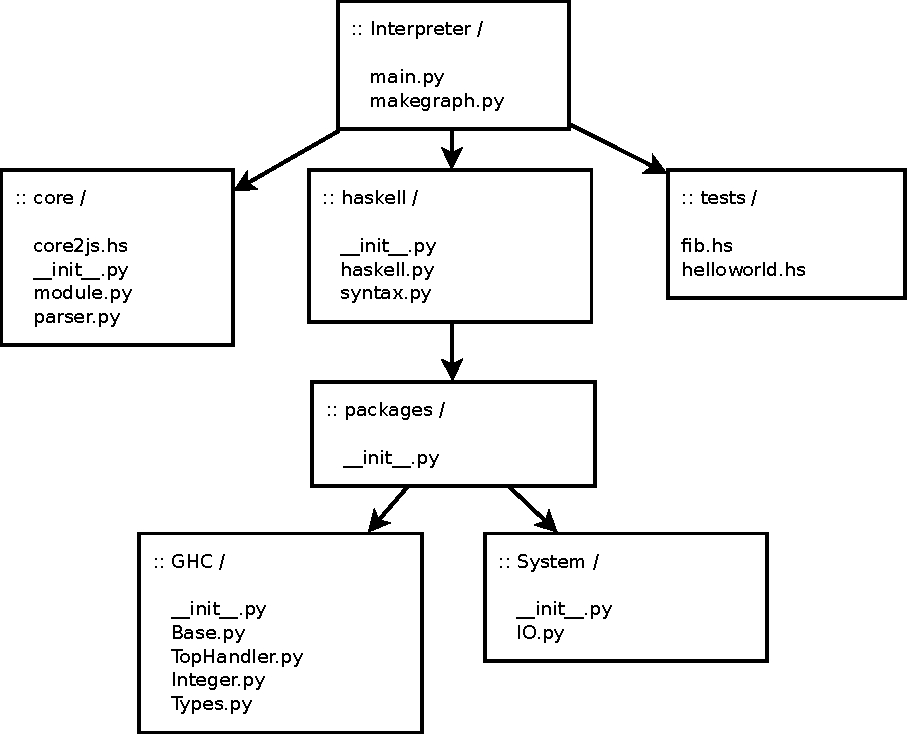
\includegraphics[width=\textwidth]{diags/organization}
\caption[Code tree: organization]{Code tree: The top of the boxes is the folder name, 
and the rest is the source files. Arrows represent subfolders.}
\label{organization}
\end{figure}

\subsection{Serializer}

The serializer consists of two parts; GHC generating External-core, and 
a Haskell program to generate JSCore (core2js.hs).

External-core is easily generated by using a compiler flag:
\begin{lstlisting}
ghc -fext-core {path-to-program}
\end{lstlisting}


The Haskell program generating JSCore uses the extcore packages. This package
implements functionality for working with External-core. The result is a datastructure
mapping directly to the External-core format defined in \cite{tolmach2010ghc}. By traversing
this structure, the program builds up a JSON tree using the Haskell JSON package.
The result is a tree of JSON constructs (corresponding to the grammar defined 
in table \ref{jscore}), this is then pretty-printed and dumped to a file.

\begin{figure}[H]
\begin{center}
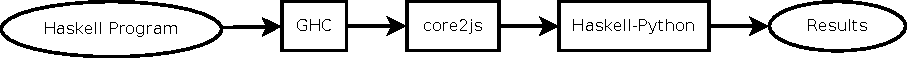
\includegraphics[width=0.3\textwidth]{diags/pipe_w_core2js}
\caption[Pipeline with core2js]{Pipeline implementation with core2js using extcore}
\label{core2js}
\end{center}
\end{figure}

\subsection{Deserializer}

The deserializer implements a JSON parser. The resulting datastructure is then 
traversed, recursively building up an AST using the constructs defined in the 
Haskell-Python interpreter. 

PyPy implements a parser generator, this simply takes a grammar defined as a 
string, written in extended-backus-naur-form (EBNF), and generates a parser. 
This parser is then used to create a JSON datastructure, as represented by 
table \ref{json}. The resulting datastructure is then traversed. By checking the 
contents of the JSON constructs with the actual JSCore format, the Core AST is built. 
External functionality is imported from the Python implementations of the Haskell 
libraries as it is encountered. 

After this is done, we are left with a "module" object, corresponding to the initial 
Haskell module. 

\subsection{Haskell libraries}

To make some simple test-cases work, some basic Haskell functionality had to be 
implemented. Some of this functionality was implemented already in the 
Haskell-Python Core' interpreter.
The work done here was mostly to organize the functionality into modules corresponding
to Haskell modules. The functionality implemented in these modules does however, 
not correspond to the Haskell implementations. This is left for future work, as this 
is a large task.

From figure \ref{helloworldgraph} (representing a "hello world" program in JSCore), 
the expression "base:SystemziIO.putStrLn" (See appendix \ref{zencoding} for a definition of
the z-encoding, used in this expression identifier) corresponds
to the Haskell function "putStrLn", which is located in the Haskell module "System.IO". 
This is translated into a reference to the function "putStrLn" defined in the python module 
"ghc.libraries.base.System.IO". See figure \ref{organization}.

\subsection{Evaluation}
\begin{sloppypar}
In order to evaluate the Haskell programs correctly, the expression "main:ZCMain.main" 
is reduced to \emph{WHNF}. However, to do this correctly would require a lot of 
the functionality used by GHC
to be implemented. Specifically, "GHC.TopHandler.runMainIO". 
In order to implement this function
a lot of other functionality would have to be implemented. 
The function is a wrapper around 
"main:Main.main", it catches uncaught exceptions and flushes stdout/stderr 
before exiting. 
\end{sloppypar}

Currently, a simple hack is implemented; the function "runMainIO" simply returns 
the function "main:Main.main".
The "main:Main.main" function is the entry-point to our program. This function 
is then evaluated when reducing "main:ZCMain.main" to WHNF.

Implementing this functionality in a manner similar to GHC is a goal for future
development. Currently, the hacks suffice for testing.
Simple Haskell functionality is implemented at a high level, such as the
"putStrLn" function which is implemented as a simple "print" Python function.

\subsection{Tests}

Testing is done by a simple Python script. The test directory has a subdirectory 
for each test. This directory
contains a Haskell program. The program is converted to External-core, then 
to JSCore, and then executed.
If the program returns "0" it passes the test. The results of running these 
tests are given in figure \ref{tests}.


\begin{figure}[H]
\begin{center}
\begin{minipage}{0.45\textwidth}
\begin{lstlisting}
-------------------------------
RESULTS
-------------------------------

factorial :  Failure
fibonacci :  Failure
helloworld :  Success
helloworld2 :  Failure
\end{lstlisting}
\end{minipage}
\end{center}
\caption[Result output from running tests]{Result output from running tests (runtests.py)}
\label{tests}
\end{figure}

The tests are supposed to be in the following increasing order of difficulty: 
helloworld, helloworld2, factorial and fibonacci. 
All the failures are due to the same problem; unimplemented 
primitives and library functions. See appendix \ref{testprograms} for test programs.

\subsection{Issues}


Very few of the initial plans regarding this project was actually realized in 
the implementation. The GHC API was intended to be used to generate JSCore, 
but this failed do to a lack of experience with Haskell and the GHC API 
(see figure \ref{haskell2js} for a description of the initially intended
pipeline). It was then discovered that a lot of the necessary code was already
written in GHC (the code that generates the External-core files), however, 
this code was not exported in any way. It was also deeply embedded in the GHC 
code. After several unfruitful attempts at creating the JSCore format by using the GHC API
and by reimplementing the GHC functions generating External-core. And some emails back 
and forth with the GHC team, these methods where abandoned.

\begin{figure}[H]
\begin{center}
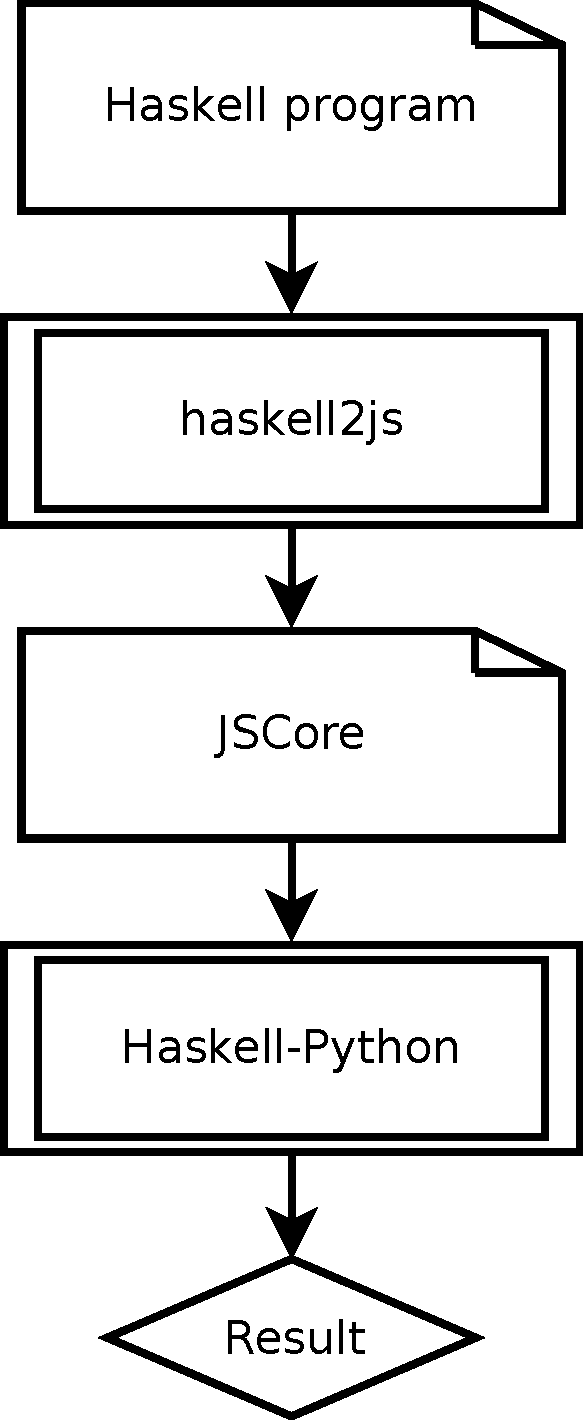
\includegraphics[width=0.3\textwidth]{diags/pipe_w_haskell2js}
\caption[Pipeline without haskell2js]{Pipeline with implementation of haskell2js using the GHC API (Not implemented)}
\label{haskell2js}
\end{center}
\end{figure}

The extcore package was then introduced, as it was thought to serve nicely for our purpose. This
does however add an extra step to the generation of JSCore, having to generate External-core
first. There is no way of working with External-core without parsing it from a file. 
See figure \ref{core2js}.

The reason for not using \emph{extcore} from the beginning was that it was thought to not be
well supported. As well as the seeming lack of support for the External-core format.

%The reason for not using \emph{extcore} from the beginning was that it was thought to not be very 
%well supported, as the External-core format seems to be changing. This also turned out to be
%the case. However, GHC also changes rapidly, and an implementation using the GHC API may not
%work for very long either. A version linking to the GHC executable would most likely be the
%worst choice. As this also changes rapidly.

A large amount of time was spent trying to generate this intermediate format. And the
greatest obstacle was that the tools being used was either incompatible, or lacking in
documentation.

The method described here worked well for very trivial Haskell programs, however, 
it turned out that
the extcore package was not able to parse any nontrivial External-core files generated 
by the GHC version used. It was thought that this was due to the fact that the extcore
package was written for earlier versions of GHC. After unsuccessfully attempting to make
the tools work with earlier versions (GHC 6.10 and 6.12 on linux and 6.10 on windows), it
turned out that the \emph{extcore} package implemented two parsers. One of which was outdated.
This was not documented anywhere, but realized after e-mailing the package maintainer, who
turned out to be very helpful.

